\documentclass{article}
\usepackage{polski}
\usepackage[utf8]{inputenc}
\usepackage{graphicx}
\usepackage[a4paper, total={7in, 10in}]{geometry}
\usepackage{listings}
\usepackage{amsmath}
\usepackage{stackengine}
\usepackage{subcaption}
\usepackage{float}
\usepackage{graphicx}
\usepackage[section]{placeins}
\graphicspath{ {./images/} }

\title{Zastosowanie Qlearningu w zachowaniu boidów}
\author{Jakub Łęcki, Marek Hering, Maciej Jabłoński}
\date{08.06.2020}
\begin{document}
\maketitle
\begin{abstract}
    Tematem niniejszej pracy jest problem nauczenia boidów (w naszym przypadku są to ryby), aby poprzez prawidłowe poruszanie się maksymalizowały swój czas życia. W tym celu użyliśmy koncepcji qlearningu oraz algorytmu stada.
\end{abstract}

\section{Boidy}
\subsection{Pochodzenie}
Termin \textbf{boid} został stworzony przez Craiga Reynoldsa w 1987 roku jako określenie stworzenia wykazującego cechy stadne. Słowo boid wzięło się z uproszeczenia terminu 'bird-like' jako odniesienie do ptaków formujących się w gromady.
\subsection{Zasady zachowania}
Okazuje się, że w świecie rzeczywistym wiele gatunków zwierząt łączących się w grupy wykazuje podobne własności. Patrząc na stada ptaków, ławice ryb, roje pszczół lub stada owiec można zauważyć, że każda z jednostek stosuje się do 3 podstawowych zasad:
\begin{enumerate}
    \item Rozdzielność - osobnik nie lubi przebywać w tłoku, dlatego zachowuje dystans do swoich sąsiadów
    \item Spójność - osobnik nie lubi przebywać w samotności, więc kieruje się ku najbliższym współstadnikom 
    \item Wyrównanie - osobnik porusza się w kierunku zbliżonym do kierunku otaczających członków stada
\end{enumerate}

Łącząc te 3 proste zasady, boidy tworzą złożone i bardzo zorganizowane skupiska, które obserwujemy jako np. ławice ryb, które pozostają w płynnym, nieustannym ruchu.
\section{Qlearning}
Jest to jedna z technik szerokiej dziedziny uczenia maszynowego znanej jako "Uczenie ze wzmocnieniem" (ang. Reinforcement Learning). Opiera się na śledzeniu zachowania agentów oraz efektów, które owe akcje powodują. W tym celu używana jest tablica stanów-akcji zwykle nazywana jako \textbf{qtable}.
\subsection{Qtable}
Tablica ma wymiary m \(\times\) n, gdzie:
\begin{itemize}
    \item m - liczba możliwych stanów
    \item n - liczba akcji możliwych do wykonania 
\end{itemize}

W każdej komórce \(Q(s,a)\) znajduje się oczekiwana wartość nagrody jaką agent otrzyma będąc w stanie \(s\) i wykonawszy akcję \(a\). Po wykonaniu akcji, agent przechodzi do kolejnego stanu \(s'\).
Agent będąc w stanie \(s\) będzie wybierać swoją kolejną akcję na podstawie polityki \(argmax(Q(s))\), czyli wybranie akcji za którą teoretycznie otrzyma największą nagrodę.
\subsection{Środowisko}
Jest to zbiór agentów oraz dowolnych innych encji z którymi agent może w jakiś sposób oddziałowywać. Rolą środowiska jest wykonanie akcji wybranej przez agenta i ocenienie jak dobrze akcja została wybrana. W tym celu środowisko nadaje agentowi nagrody (i kary, jeśli nagroda jest ujemna). W kolejnych rundach skutkuje to stopniowym poprawianiem procesu wyboru akcji i agent zbiera coraz wyższe nagrody. Po wykonaniu kroku środowisko przekazuje do algorytmu uczenia zestaw danych:
\begin{itemize}
    \item stan w którym był agent
    \item akcja jaką wykonał
    \item stan w którym znajduje się po wykonaniu akcji
    \item nagroda jaką otrzymał za przejście do kolejnego stanu
\end{itemize}
\subsection{Proces uczenia}
Aby agent wybierał z czasem coraz lepsze decyzje, wartości w Qtable muszą ulegać zmianie. Odbywa się to w oparciu o poniższe równanie:
\begin{equation}
    \label{eqn:bellman_equation}
    Q'(s, a)\leftarrow Q(s, a) + \alpha \cdot\left(r  + \gamma\cdot \stackunder{max}{a} Q(s', a) - Q(s,a) \right) 
\end{equation}
Gdzie \(s\) i \(a\) to stan i akcja przed jej wykonaniem, a  \(s'\) to stan po wykonaniu akcji.
\subsubsection{Współczynnik uczenia \(\alpha\)}
Wartość \(\alpha \in <0, 1>\) reguluje jak bardzo znacząca jest nowa informacja uzyskana w wyniku wykonania akcji w środowisku. Przy wartości 0 agent nie będzie się uczył niczego nowego, natomiast przy \(\alpha = 1\) agent zaakceptuje całą zdobytą wiedzę. 
\subsubsection{Współczynnik dyskontowania \(\gamma\)}
Wartość \(\gamma \in <0, 1>\) określa ważność przyszłych nagród zdobywanych przez agenta. Wartość dążąca do zera zwiększy sugerowanie się pamięcią krótkotrwałą, natomiast do 1 pamięcią długotrwałą. Ważnym elementem jest, aby \(\gamma\) rzeczywiście zawierała się w przedziale \(<0, 1)\) ponieważ zapewnia to zbieżność wartości przewidywanej nagrody. Jeśli proces uczenia byłby nieskończony i \(\gamma \ge 1\) (a nawet lekko poniżej) wartości nagród rosłyby nieustannie zaburzając proces.
\subsubsection{Efekt}
W wyniku przeprowadzenia odpowiedniej ilości kroków wartości nagród zbiegają się do optymalnych, a w tabeli powstają zależności pomiędzy poszczególnymi stanami umożliwiające dotrzeć do nawiększej nagrody, dysponując jedynie obecnym stanem i przewidywaną nagrodą.
\subsubsection{Polityka wspomagająca}
Gdy podczas uczenia agent będzie słuchał się tylko tabeli qlearningu, może się zdarzyć że zadowoli się częściowo poprawnym rozwiązaniem, zamiast szukać rozwiązania dokładnego. Aby uniknąc takiej sytuacji proces wybierania akcji rozszerza się często o politykę \textbf{epsilon greedy}, w której z pewnym prawdopodobieństwem wybierana jest losowa akcja zamiast wskazywanej przez tabelę. Wartość \(\epsilon\) jest zmniejszana z czasem, aby agent coraz częściej stosował to czego się nauczył.

\section{Kontrola ruchu boidów}
\subsection{Ruch ciągły}
Boidy muszą być osadzone w przestrzeni euklidesowej, zatem każdy z boidów posiada trzy dwuwymiarowe wektory położenia, prędkości i przyspieszenia.\\
Aby agent mógł poruszać się ruchem gładkim, postanowiliśmy kontrolować boidy za pomocą przyspieszenia, a na prędkość nałożyć ograniczenia w postaci minimalnej i maksymalnej wartości.
\subsection{Stan agenta}
Stanem agenta jest jego pozycja oraz kąt nachylenia prędkości do osi X. 
\subsection{Dyskretyzacja}
Qlearning z definicji działa na wartościach dyskretnych, ponieważ wartości nagród wpisujemy pod konkretne wiersze i kolumny tabeli. Zatem konieczne było zdyskretyzowanie stanu agenta. Wykonaliśmy to poprzez przeniesienie pozycji agenta w przestrzeń o dużo mniejszej rozdzielczości \(r\), a kąt spłaszczamy do \(N\) równo oddalonych wartości.
\subsection{Akcja agenta}
W klasycznym algorytmie qlearningu na wyjściu otrzymujemy \(N\) wartości nagród, spośród których indeks maksymalnej wartości symbolizuje akcję do wykonania. W naszym problemie jednak sprowadzenie ruchu do zaledwie kilku kierunków nie spełniłoby założenia o gładkości, dlatego przyjęliśmy nową politykę. Zamiast wyznaczać przyśpieszenie na podstawie jednej akcji, wyznaczamy je według wzoru:
\begin{equation}
    a = \sum \limits_{i = 0}^{N}a_i
\end{equation}
gdzie \(i\) to indeks akcji, \(N\) to ilość możliwych kierunków, natomiast \(a_i\) to wektor w postaci biegunowej: 
\begin{equation}
    a_i = [r_i, i \cdot 360/N]
\end{equation}
gdzie \(r_i\) to wartość nagrody otrzymanej za i-tą akcję.\\
Użycie wartości nagrody poskutkuje poprawną reakcją boida ponieważ w miejscach których ma unikać nagroda będzie ujemna, a w możliwych do przemieszczenia - dodatnia.
\section{Utrzymanie agentów na planszy}

\begin{figure}[H]
    \centering
    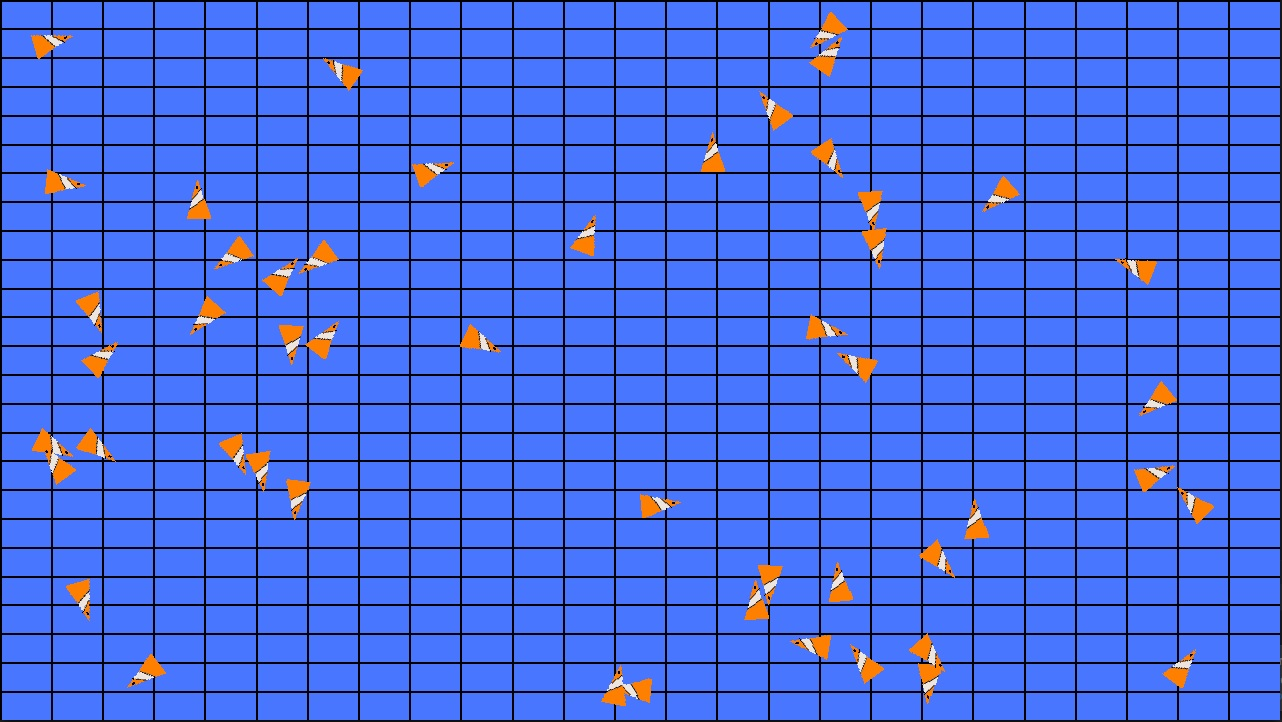
\includegraphics[width=0.75\textwidth]{1_Qtable_init.jpg}
    \caption[]{Stan początkowy planszy z agentami. Siatka symbolizuje komórki qtable zależne od położenia}
\end{figure}
Na początku zajęliśmy się nauczeniem boidów, aby nie dotykały krawędzi. W tym celu przyjęliśmy rozdzielczość tablicy stanów \(25\times25\) oraz 12 kierunków w których możliwe jest obliczenie przyśpieszenia.\\
Dodatkowo:
\begin{enumerate}
    \item ilość ryb = 50
    \item długość epoki = 2000 klatek (\(\approx\) 1 min)
\end{enumerate}
\subsection{Nagradzanie}
Boid za dotknięcie granicy otrzymuje nagrodę o wysokości -1000.
\subsection{Wynik}
Boidy dość skutecznie utrzymywały się przy życiu, jednak ich ruch bardziej przypominał odbijanie się niż omijanie krawędzi. Wynika to z faktu, że nagroda wyznaczana jest tylko w tej komórce w której agent zginie, nie ma żadnej relacji pomiędzy sąsiednimi stanami, więc reakcja następowała tylko tuż przy granicy.
\subsection{Modyfikacja polityki aktualizacji tablicy stanów}
W tradycyjnym algorytmie qlearningu, równanie (\ref{eqn:bellman_equation}) Bellmana aktualizuje stan przez wybranie maksymalnej nagrody możliwej do uzyskania. W naszym przypadku nie jest to skuteczne, ponieważ wykonanie akcji nie skutkuje natychmiastowym uzyskaniem nagrody. Aby umożliwić agentowi ocenienie czy warto ruszyć się w danym kierunku zrezygnowaliśmy z wybierania wartości maksymalnej. Zamiast tego bierzemy wszystkie możliwe nagrody do uzyskania po wyjściu z obecnego stanu i liczymy średnią arytmetyczną z minimalnej i maksymalnej nagrody. Dzięki temu w tabeli stanów powstaje swego rodzaju dyskretne pole siłowe, które nadaje boidom kierunek w którym powinny się udać.
\subsection{Stan tabeli z nową polityką nagród} 
Po powyższej zmianie wyniki mają się następująco. Strzałki oznaczają kierunek wypadkowego przyśpieszenia.

\begin{figure}[H]
    \begin{minipage}[h]{0.48\textwidth}
        \centering
        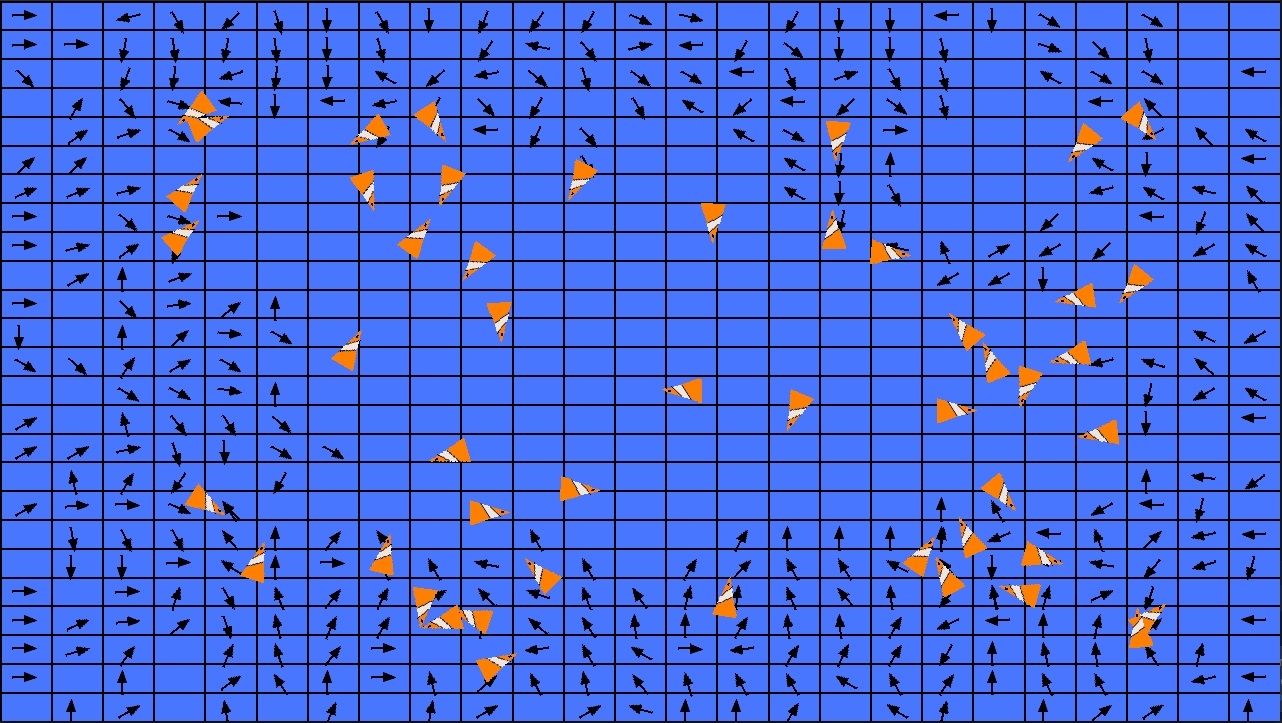
\includegraphics[width=\textwidth]{2_Qtable_after_2nd_epoch.jpg}
        \caption{Stan tabeli po dwóch epokach}
    \end{minipage}
    \hspace{0.02\textwidth}
    \begin{minipage}[h]{0.48\textwidth}
        \centering
        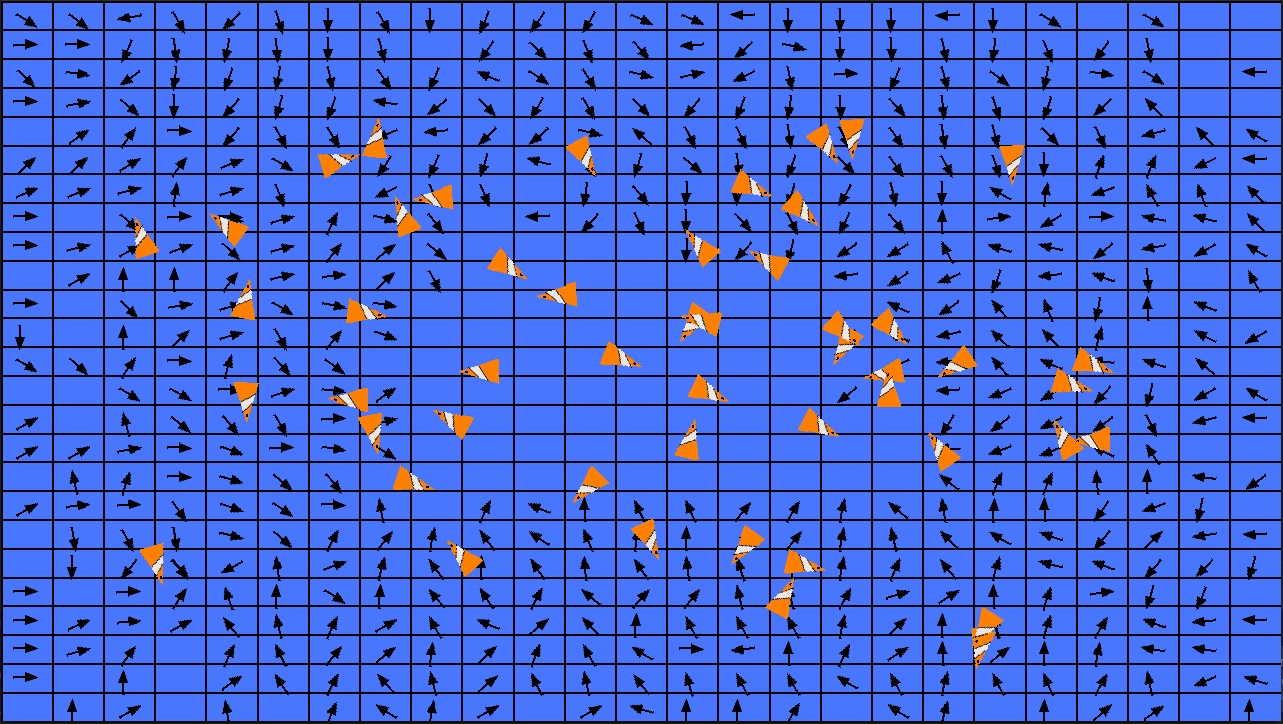
\includegraphics[width=\textwidth]{3_Qtable_after_3rd_epoch.jpg}    
        \caption{Stan tabeli po 3 epokach}
    \end{minipage}
\end{figure}
\begin{figure}[H]
    \begin{minipage}[h]{0.48\textwidth}
        \centering
        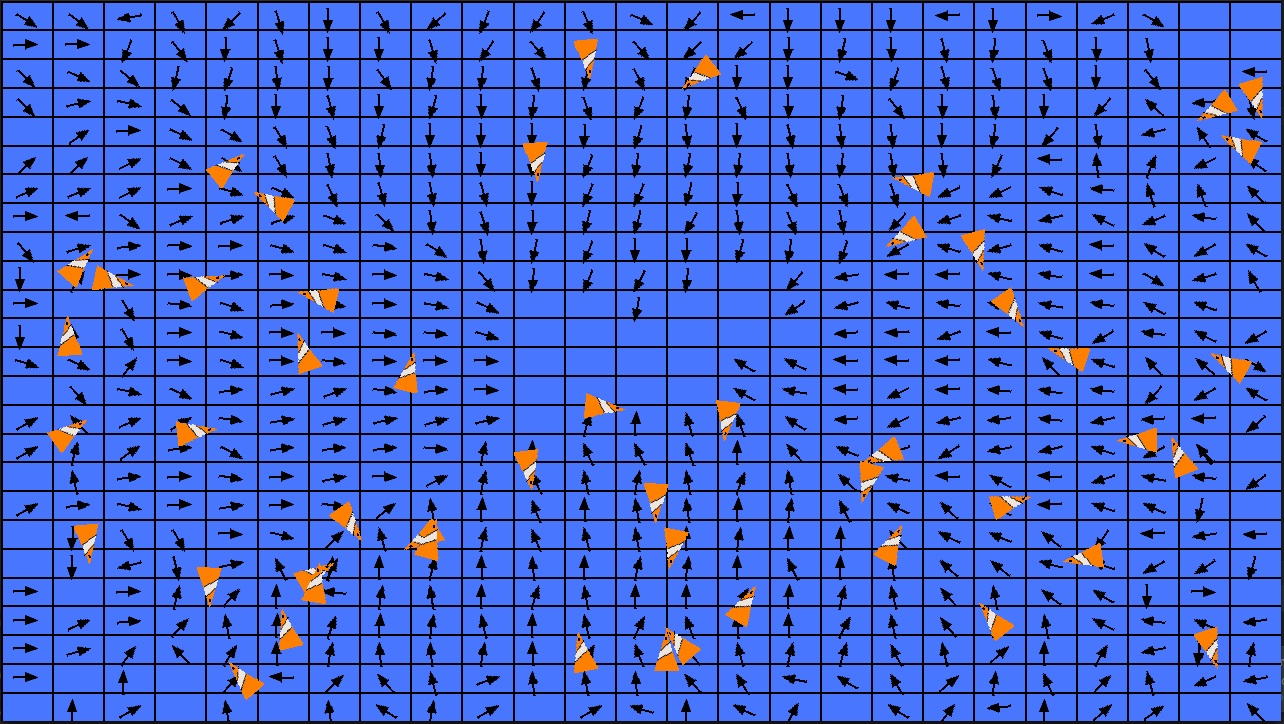
\includegraphics[width=\textwidth]{4_Qtable_after_5rd_epoch.jpg}
        \caption{Stan tabeli po 5 epokach}
    \end{minipage}
    \hspace{0.02\textwidth}
    \begin{minipage}[h]{0.48\textwidth}
        \centering
        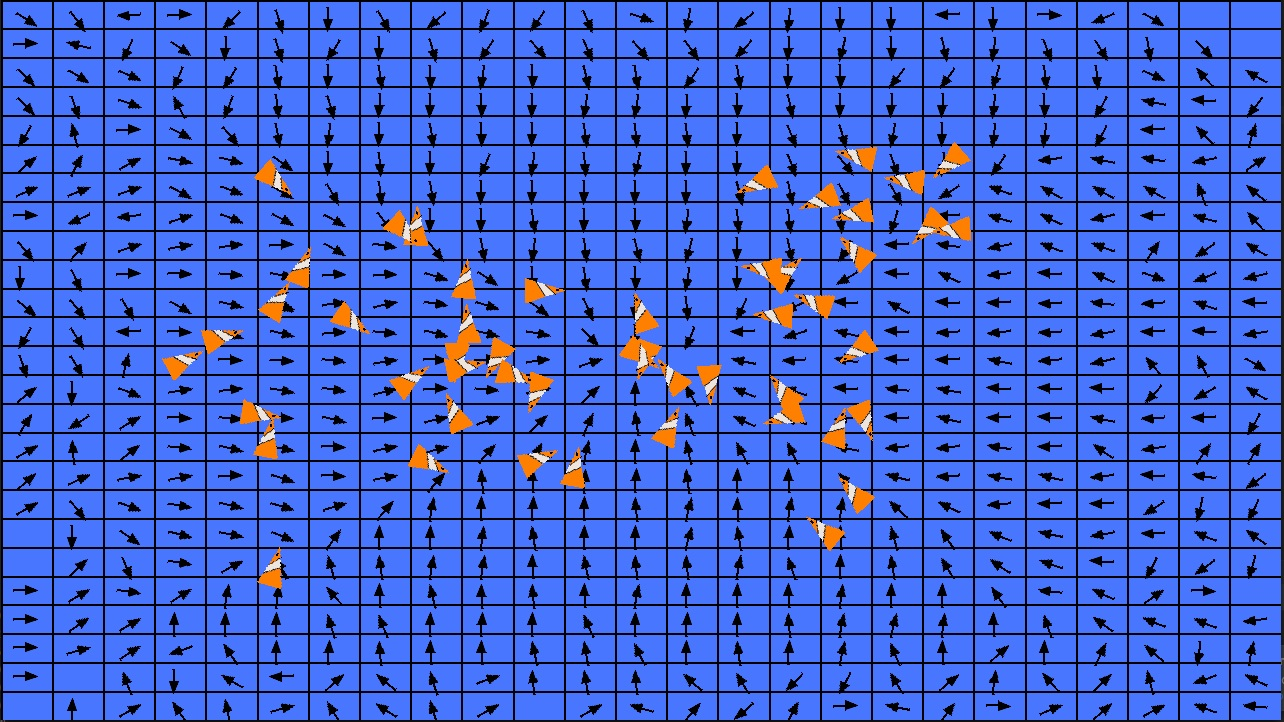
\includegraphics[width=\textwidth]{5_Qtable_after_10th_epoch.jpg}
        \caption{Stan tabeli po 10 epokach}
    \end{minipage}
\end{figure}

Jak widać już po 10 epokach agenci nauczyli się skutecznie unikać krawędzi. Patrząc na kierunki poszczególnych strzałek widzimy, że w tabeli powstało pole, które zbiega się do środka tworząc optymalne ścieżki nawet w nietrywialnych miejscach takich jak rogi planszy. Jest to bardzo korzystne, ponieważ takie miejsca sprawiają zawsze problem w alogorytmicznym wykrywaniu kolizji.

\begin{figure}[H]
    \begin{minipage}{0.48\textwidth}
        \centering
        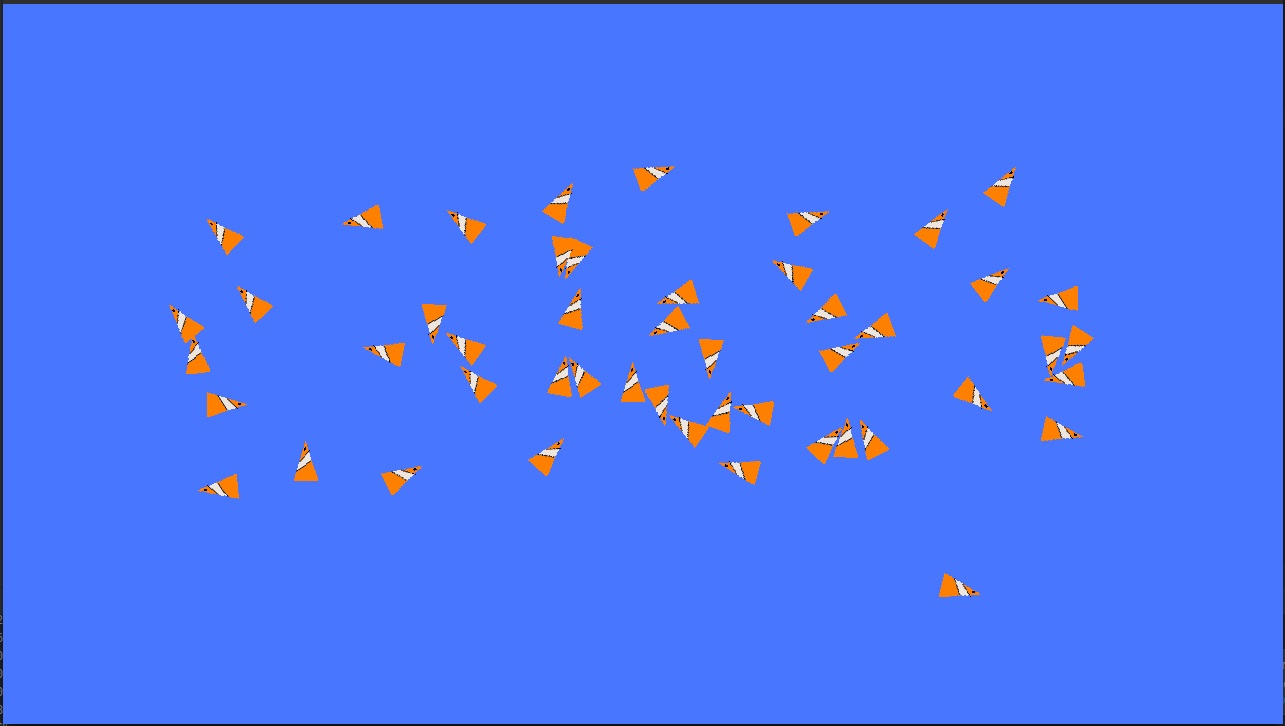
\includegraphics[width=\textwidth]{6_Learing_result.jpg}
        \caption{Ryby utrzymujące się na środku planszy po nauczeniu}
    \end{minipage}
    \hspace{0.02\textwidth}
    \begin{minipage}{0.48\textwidth}
        \centering
        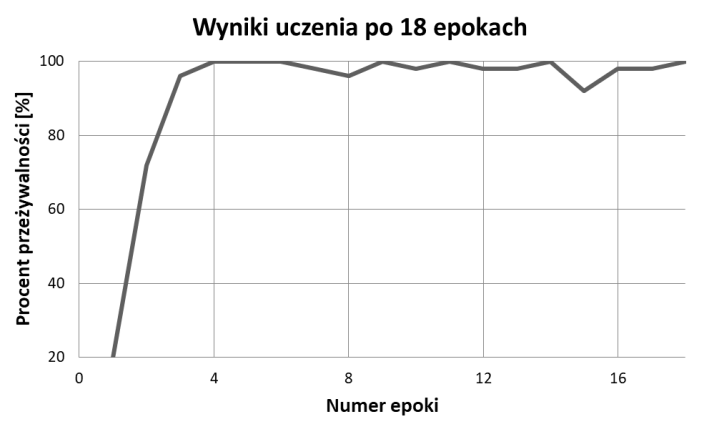
\includegraphics[width=\textwidth]{borders_learning_plot.png}
        \caption{Wykres przeżywalności ryb w czasie uczenia}
    \end{minipage}
\end{figure}
\section{Polowanie i uciekanie}
W kolejnym etapie postanowiliśmy dodać do środowiska boidy drugiego rodzaju, tzn. drapieżniki. Ich zadaniem jest manipulowanie swoim ruchem, aby zjadać ryby. W momencie kolizji drapieżnika z rybą następuje śmierć ryby. Drapieżniki tak samo jak ryby umierają na krawędziach planszy.
\subsection{Qtable}
Aby umożliwić nauczenie się zarówno uciekania jak i gonienia rozszerzyliśmy tablicę stanów o 2 wymiary. Jeden który indeksuje rodzaj uczącego się boida, drugi natomiast zawiera stany jako dyskretny kąt pod którym agent widzi swój cel. Celem odpowiednio jest najbliższa ryba dla drapieżnika i najbliższy drapieżnik dla ryby.
\subsection{Pole reakcji}
Odnajdywanie najbliższego celu dla każdego boida na planszy ma istotne wady.
\begin{enumerate}
    \item Jest wysoce nieoptymalne, ponieważ wymaga przeszukania każdy z każdym więc ma czas \(O(n^2)\)
    \item Sugeruje, że boid posiada wiedzę \textit{a priori} o położeniu dowolnego innego boida, co nie pokrywa się z rzeczywistością, gdzie każdy organizm ma ograniczone pole widzenia i reakcji.
\end{enumerate}
\end{document}